\documentclass[a4paper,openright,12pt]{report}

%
% Times New Roman font.
%
\usefont{T1}{ptm}{m}{n}
\selectfont


% Packages a utilizar e respetivos parâmetros.
\usepackage{inputenc}
\usepackage{enumitem}
\usepackage[english]{babel}
\usepackage{graphicx}
\usepackage{url}
\usepackage{anyfontsize}
% Definições das dimensões das páginas
\setlength{\textheight}{24.00cm}
\setlength{\textwidth}{15.50cm}
\setlength{\topmargin}{0.35cm}
\setlength{\headheight}{0cm}
\setlength{\headsep}{0cm}
\setlength{\oddsidemargin}{0.25cm}
\setlength{\evensidemargin}{0.25cm}

%
% Times New Roman font.
%
\usefont{T1}{ptm}{m}{n}
\selectfont

%
%title
%
\title{%
  \vspace{-50mm}
  \begin{minipage}[l]{150mm}
    \resizebox{50mm}{!}{
\includegraphics{./figures/logo_isel.png}}
  \end{minipage}\\
  \vspace{20mm}
  \textbf{Proposta de Projeto}
}

%
%authors
%
\author{%
  \begin{tabular}{ll}
      & David Fildago \\
      & goncalo9marco@hotmail.com\\
      & 968 225 962
  \\ \\
    & Pedro Santos \\
    & santos.pedroc@gmail.com \\
    & 962 942 930
  \\ \\
    & Valdemar Antunes \\
    & ValdemarPCA@hotmail.com \\
    & 966 439 259
  \end{tabular}
} 

%
% date
% 
\date{%
\vspace{30mm}
\begin{tabular}{ll}
  \centering
  & {Orientadores:} \\
  & *Paula Graça, ISEL, paula.graca@isel.pt* \\
  & *Diogo Pacheco, Do iT Lean, diogo.pacheco@doitlean.com*\\
\end{tabular}\\
\vspace{20mm}
Proposta de projeto realizado no âmbito de Projecto e Seminário,\\
do curso de licenciatura em Engenharia Informática e de Computadores\\
Semestre de Verão 2019/2020
\vspace{20mm}\\
14 de Março de 2020}

\begin{document}
\thispagestyle{empty}
\maketitle
\section*{Introduction}
 Today's market, increasingly technological, demanding and challenging, imposes a work rhythm on companies that besides managing their core business processes, also have a significant amount of dynamics on internal activities to help them in their growth and competitiveness. In particular, companies in the information and technologies sector keep internal activities such as work fairs, knowledge sharing through informal presentations, software components development, qualification opportunities, playful activities, among others. To put these activities in practise in an efficient way, there must exist a coordination of resources that is not easy to obtain, given its allocation to ongoing projects. \par
    However, by developing a collaboration platform we can achieve a correct management of the plannings so that they can be executed in due time, and the whole process can be agiled allowing not only the registration and publication of internal needs, but also the acceptance of applications by the colaborators interested in its development. Therefore, it is intended to develop a web reactive application using the OutSystems platform, that functions as a collaboration platform designed for the management of internal corporate necessities in a company, and is accesible in all kinds of devices: browsers, tablets and smartphones.
    
    
\section*{Requirements}

In order to create a fully functional, efficient and trustworthy reactive web application that will work as a collaboration platform for companies to use, there must be a set of requirements that are predefined in due time. The understanding of the OutSystems platform and the exploration of its usability is a key factor that will provide a concise implementation of these requirements. The main requirements are described as:
  
\begin{enumerate}
\item Registration and authentication in the collaboration platform.
\item Registration of the company's internal necessities, such as the planning of events or job faires, informal meetings with the goal of sharing knowledge between employees, right medium posts, qualification offers, software components development, internal oportunities for career progress and off work activities.
\item Disclosure and scheduling of the company's necessities.
\item Application management and registration for the divulged necessities.
\item Create notifications targeting the author of the necessity when there are new applications and targeting candidates when their application has been accepted or refused, as well as uppon the application's closure.
\item Possibility of integrating the collaboration platform with Google Maps in order to mark/indicate the place for events that take place outside of the company.
\end{enumerate}

There were defined optional requirements, to be implemented according to how the main requirements are fulfilled. These are defined as:

\begin{enumerate}
\item Generation of reports that are defined according to how the internal needs of the company/events were fulfilled.
\item Registration of who applies the most to what kinds of events or internal needs, creating a top three or top five representation for each event/internal need. 
\item Individual indication of presence or arrival at the place of an event, that can be observed by other participants.
\end{enumerate}

\section*{Schedule} 

The project's management and schedule (fig. 1) will follow an agile [1] designated methodology, where the SCRUM framework [2] will be used since it is the most well referenced and it enables to increase the productivty and quality of the development. Consequently, the project will be divided in cycles called Sprints, where the development of the project is focused on concluding an incremental solution that results from a previously established objective. Each incremental solution  is a fully functional, integrated, tested and documented application in which the final sprint will correspond to the delivery of the final product. In Figure 1 bellow, we can verify the schedule of all the sprints and phases included in the project.

\begin{figure}[h]
  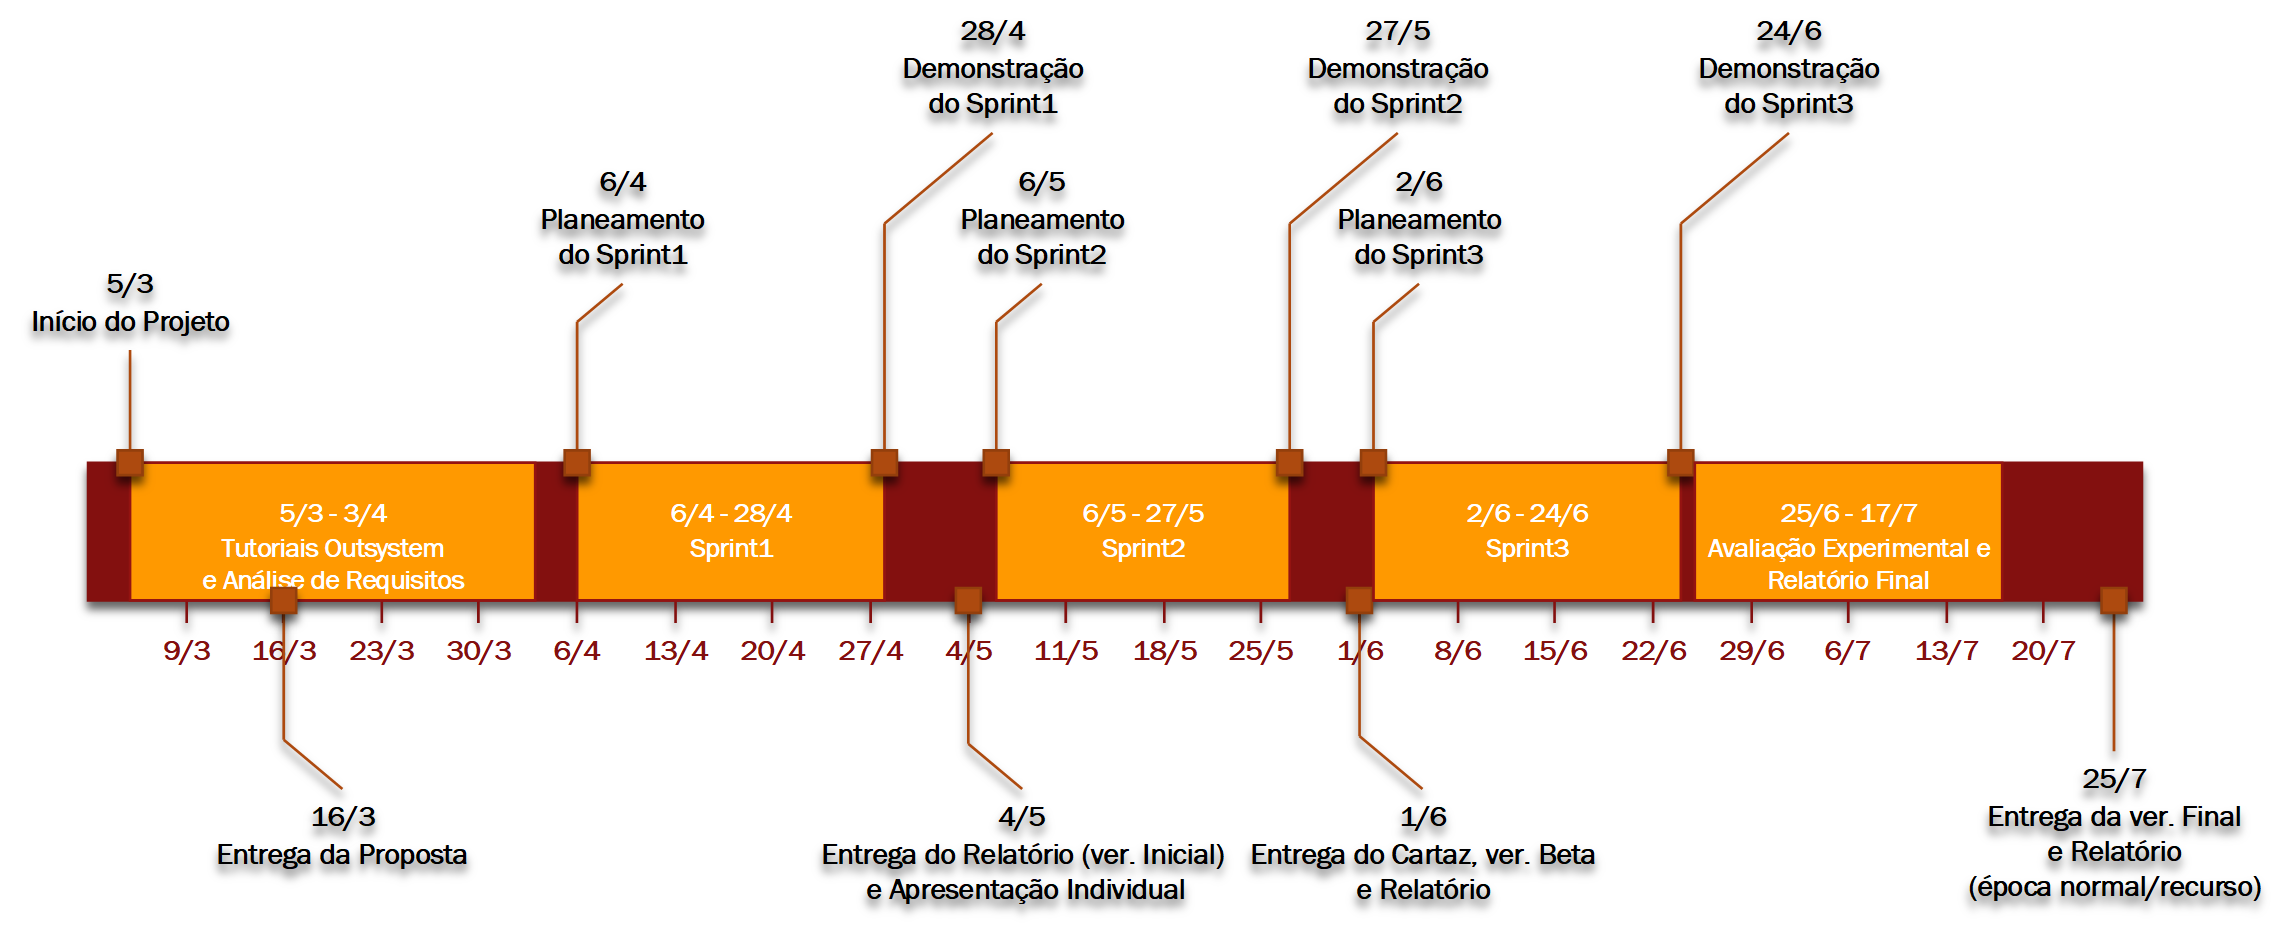
\includegraphics[width=\linewidth]{./figures/Timeline Projeto LEIC.png}
  \caption{Project Timeline}\label{fig:schedule}
\end{figure}

The initial phase of the project's development consists in making the Outsystems tutorials followed by a requirements analysis. The sprints that will be made whilst the development of the project will start with it's planning and end with a demonstration and the elaboration of the project's report which will be made progressively throughout the sprints.

\section*{References}
\begin{enumerate}[label={[\arabic*]}]
  \item https://www.agilealliance.org/agile101/the-agile-manifesto
  \item https://www.scrum.org/resources/scrum-guide
\end{enumerate}

\end{document}